\chapter{Implementacja}
\label{cha:implementation}

W niniejszym rozdziale przedstawiono szczegóły implementacyjne zrealizowanego systemu generatora danych syntetycznych. Opisano architekturę rozwiązania, zastosowane technologie oraz kluczowe komponenty zarówno po stronie serwera (backend), jak i klienta (frontend). Przedstawiono również sposób konfiguracji środowiska uruchomieniowego oraz proces wdrażania aplikacji przy użyciu konteneryzacji.

\section{Architektura systemu}
System został zaprojektowany w architekturze klient-serwer, z wyraźnym podziałem na warstwę prezentacji (frontend) oraz warstwę logiki biznesowej i dostępu do danych (backend). Komunikacja między tymi warstwami odbywa się za pośrednictwem interfejsu \gls{REST} \gls{API} \cite{rest_fielding}. Całość systemu została skonteneryzowana przy użyciu platformy Docker, co zapewnia łatwość wdrożenia i spójność środowiska uruchomieniowego. Poniżej przedstawiono schemat architektury systemu (Rysunek \ref{fig:architecture_diagram}).

\begin{figure}[H]
    \centering
    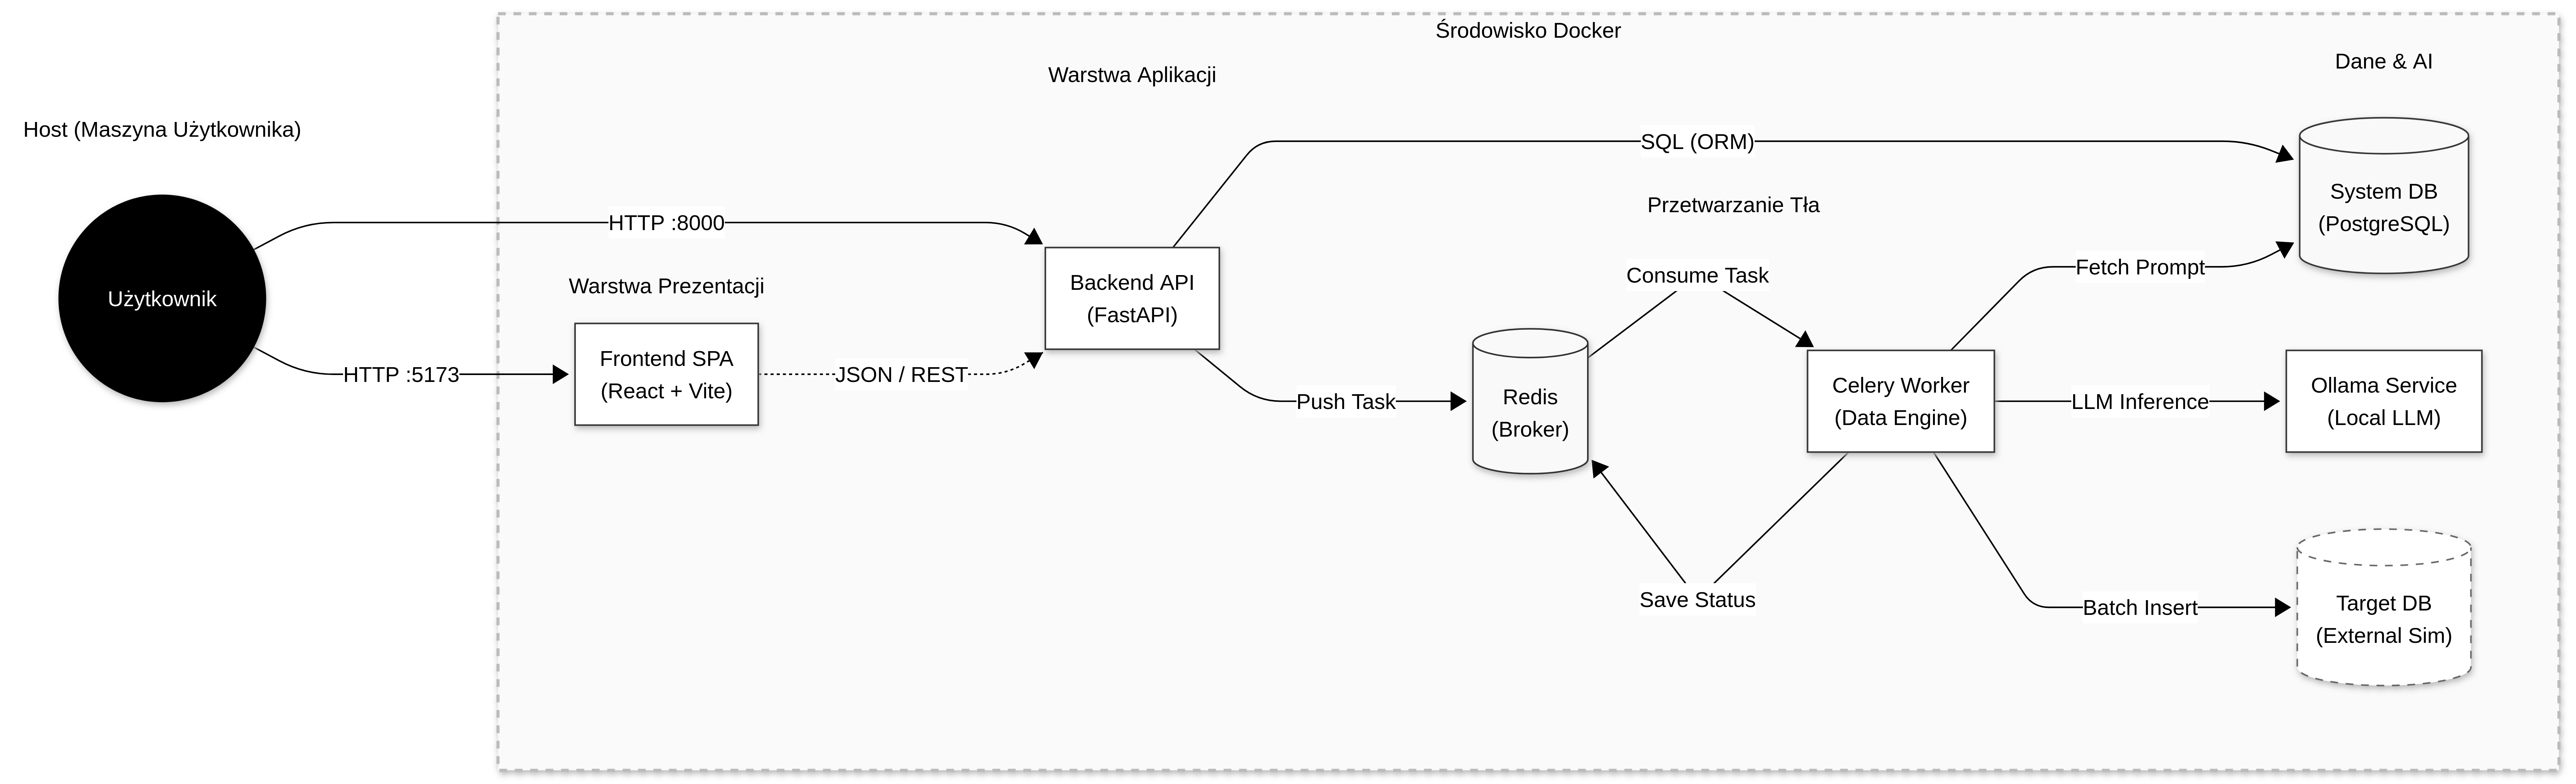
\includegraphics[width=1\textwidth]{images/docker_diagram.png}
    \caption{Schemat architektury systemu}
    \label{fig:architecture_diagram}
\end{figure}

Główne elementy systemu to:
\begin{itemize}
    \item Backend \gls{API}: Serwer aplikacji odpowiedzialny za logikę biznesową, autentykację użytkowników oraz zarządzanie procesem generowania danych.
    \item Frontend: Aplikacja internetowa umożliwiająca użytkownikom interakcję z systemem, definiowanie schematów danych oraz podgląd wyników.
    \item Baza danych (PostgreSQL): Przechowuje informacje o użytkownikach, projektach oraz historię zadań.
    \item Kolejka zadań (Redis): Pośredniczy w przekazywaniu zadań generowania danych do procesów roboczych (workerów), co pozwala na asynchroniczne przetwarzanie długotrwałych operacji.
    \item Worker (Celery): Proces odpowiedzialny za właściwe generowanie danych na podstawie zdefiniowanych reguł.
    \item Ollama (\gls{LLM}): Lokalny serwer modeli językowych, wykorzystywany do generowania danych wymagających kreatywności i kontekstu \cite{ollama}.
\end{itemize}

\section{Implementacja backendowa}
Warstwa backendowa została zaimplementowana w języku Python, z wykorzystaniem frameworka FastAPI. Wybór ten podyktowany był wysoką wydajnością FastAPI, wbudowaną obsługą asynchroniczności oraz automatycznym generowaniem dokumentacji \gls{API} (Swagger \gls{UI}).

\subsection*{Struktura projektu}
Kod źródłowy backendu został podzielony na moduły zgodnie z zasadą pojedynczej odpowiedzialności:
\begin{itemize}
    \item \texttt{main.py}: Punkt wejścia aplikacji, konfiguracja serwera i definicja tras \gls{API}.
    \item \texttt{models.py}: Modele danych Pydantic służące do walidacji żądań i odpowiedzi \gls{API}.
    \item \texttt{database.py}: Konfiguracja połączenia z bazą danych przy użyciu biblioteki SQLAlchemy.
    \item \texttt{engine.py}: Główny silnik generowania danych.
    \item \texttt{tasks.py}: Definicje zadań asynchronicznych dla Celery.
    \item \texttt{auth.py}: Logika uwierzytelniania i autoryzacji (OAuth2, haszowanie haseł).
\end{itemize}

\subsection*{Silnik generowania danych (Data Engine)}
Sercem systemu jest klasa \texttt{DataEngine} znajdująca się w pliku \texttt{engine.py}. Odpowiada ona za interpretację schematu danych zdefiniowanego przez użytkownika i fizyczne wygenerowanie wartości dla poszczególnych pól.

Kluczowym wyzwaniem implementacyjnym było obsłużenie zależności między tabelami (klucze obce). W tym celu zaimplementowano metodę \texttt{\_resolve\_generation\_order}, która analizuje graf zależności między tabelami i ustala poprawną kolejność generowania. Algorytm ten zapewnia, że dane do tabeli nadrzędnej są generowane przed danymi do tabeli podrzędnej.

Generowanie wartości dla poszczególnych pól realizowane jest przez dedykowane metody:
\begin{itemize}
    \item \texttt{\_generate\_template\_value}: Pozwala na tworzenie wartości pochodnych przy użyciu szablonów Jinja2, bazując na innych polach w tej samej tabeli.
    \item \texttt{\_generate\_regex\_value}: Generuje ciągi znaków pasujące do podanego wyrażenia regularnego, wykorzystując bibliotekę \texttt{rstr}.
    \item \texttt{\_generate\_timestamp\_value}: Generuje losowe daty i czasy w określonym przedziale.
    \item \texttt{\_generate\_integer\_or\_float\_value}: Generuje liczby całkowite lub zmiennoprzecinkowe w zadanym zakresie.
    \item \texttt{\_generate\_boolean\_value}: Zwraca wartość logiczną prawda/fałsz z określonym prawdopodobieństwem.
    \item \texttt{\_generate\_faker\_value}: Wykorzystuje bibliotekę \texttt{Faker} do tworzenia realistycznych danych (imiona, adresy, emaile).
    \item \texttt{\_generate\_distribution\_value}: Losuje wartość z podanej listy opcji z uwzględnieniem rozkładu prawdopodobieństwa.
    \item \texttt{\_generate\_foreign\_key\_value}: Rozwiązuje relacje między tabelami, pobierając identyfikator z innej, wcześniej wygenerowanej tabeli.
    \item \texttt{\_generate\_llm\_value}: Komunikuje się z modelem językowym (przez OpenAI \gls{API} lub lokalną instancję Ollama) w celu wygenerowania danych kontekstowych.
\end{itemize}

\subsection*{Przetwarzanie asynchroniczne}
Ze względu na potencjalnie długi czas generowania dużych zbiorów danych, proces ten został odseparowany od głównego wątku obsługi żądań \gls{HTTP}. Wykorzystano w tym celu bibliotekę Celery oraz bazę Redis jako brokera wiadomości.

Użytkownik, zlecając generowanie danych, wysyła żądanie do endpointu \texttt{/generate/async}. System tworzy nowe zadanie, zwraca identyfikator \texttt{job\_id} i kończy obsługę żądania \gls{HTTP}. Właściwe generowanie odbywa się w tle przez proces Workera. Status zadania jest monitorowany przez klienta w czasie rzeczywistym za pomocą protokołu WebSocket (endpoint \texttt{/ws/jobs/\{job\_id\}}), co pozwala na wyświetlanie paska postępu.

\subsection*{Bezpieczeństwo}
System implementuje mechanizm uwierzytelniania oparty na tokenach \gls{JWT} \cite{jwt_rf7519}. Hasła użytkowników są bezpiecznie przechowywane w bazie danych w formie zahaszowanej (przy użyciu algorytmu bcrypt). Każdy chroniony endpoint \gls{API} weryfikuje ważność tokenu przed przetworzeniem żądania, co realizowane jest za pomocą mechanizmu Dependency Injection w FastAPI.

\section{Implementacja frontendowa}
Warstwa prezentacji została zrealizowana jako aplikacja typu Single Page Application (\gls{SPA}) przy użyciu biblioteki React. Do budowania projektu wykorzystano narzędzie Vite, a za stylowanie odpowiada framework Tailwind \gls{CSS}.

\subsection*{Szczegółowy opis interfejsu}
W dalszej części tego rozdziału przedstawiono kluczowe elementy interfejsu graficznego aplikacji. Interfejs został zaprojektowany w sposób minimalistyczny, z wykorzystaniem ciemnego motywu, aby zapewnić komfort pracy przy długotrwałym użytkowaniu. Aplikacja jest w języku angielskim, co jest standardem w narzędziach deweloperskich.

\subsection*{Ekran logowania}
Dostęp do systemu jest chroniony i wymaga uwierzytelnienia.
\begin{figure}[H]
    \centering
    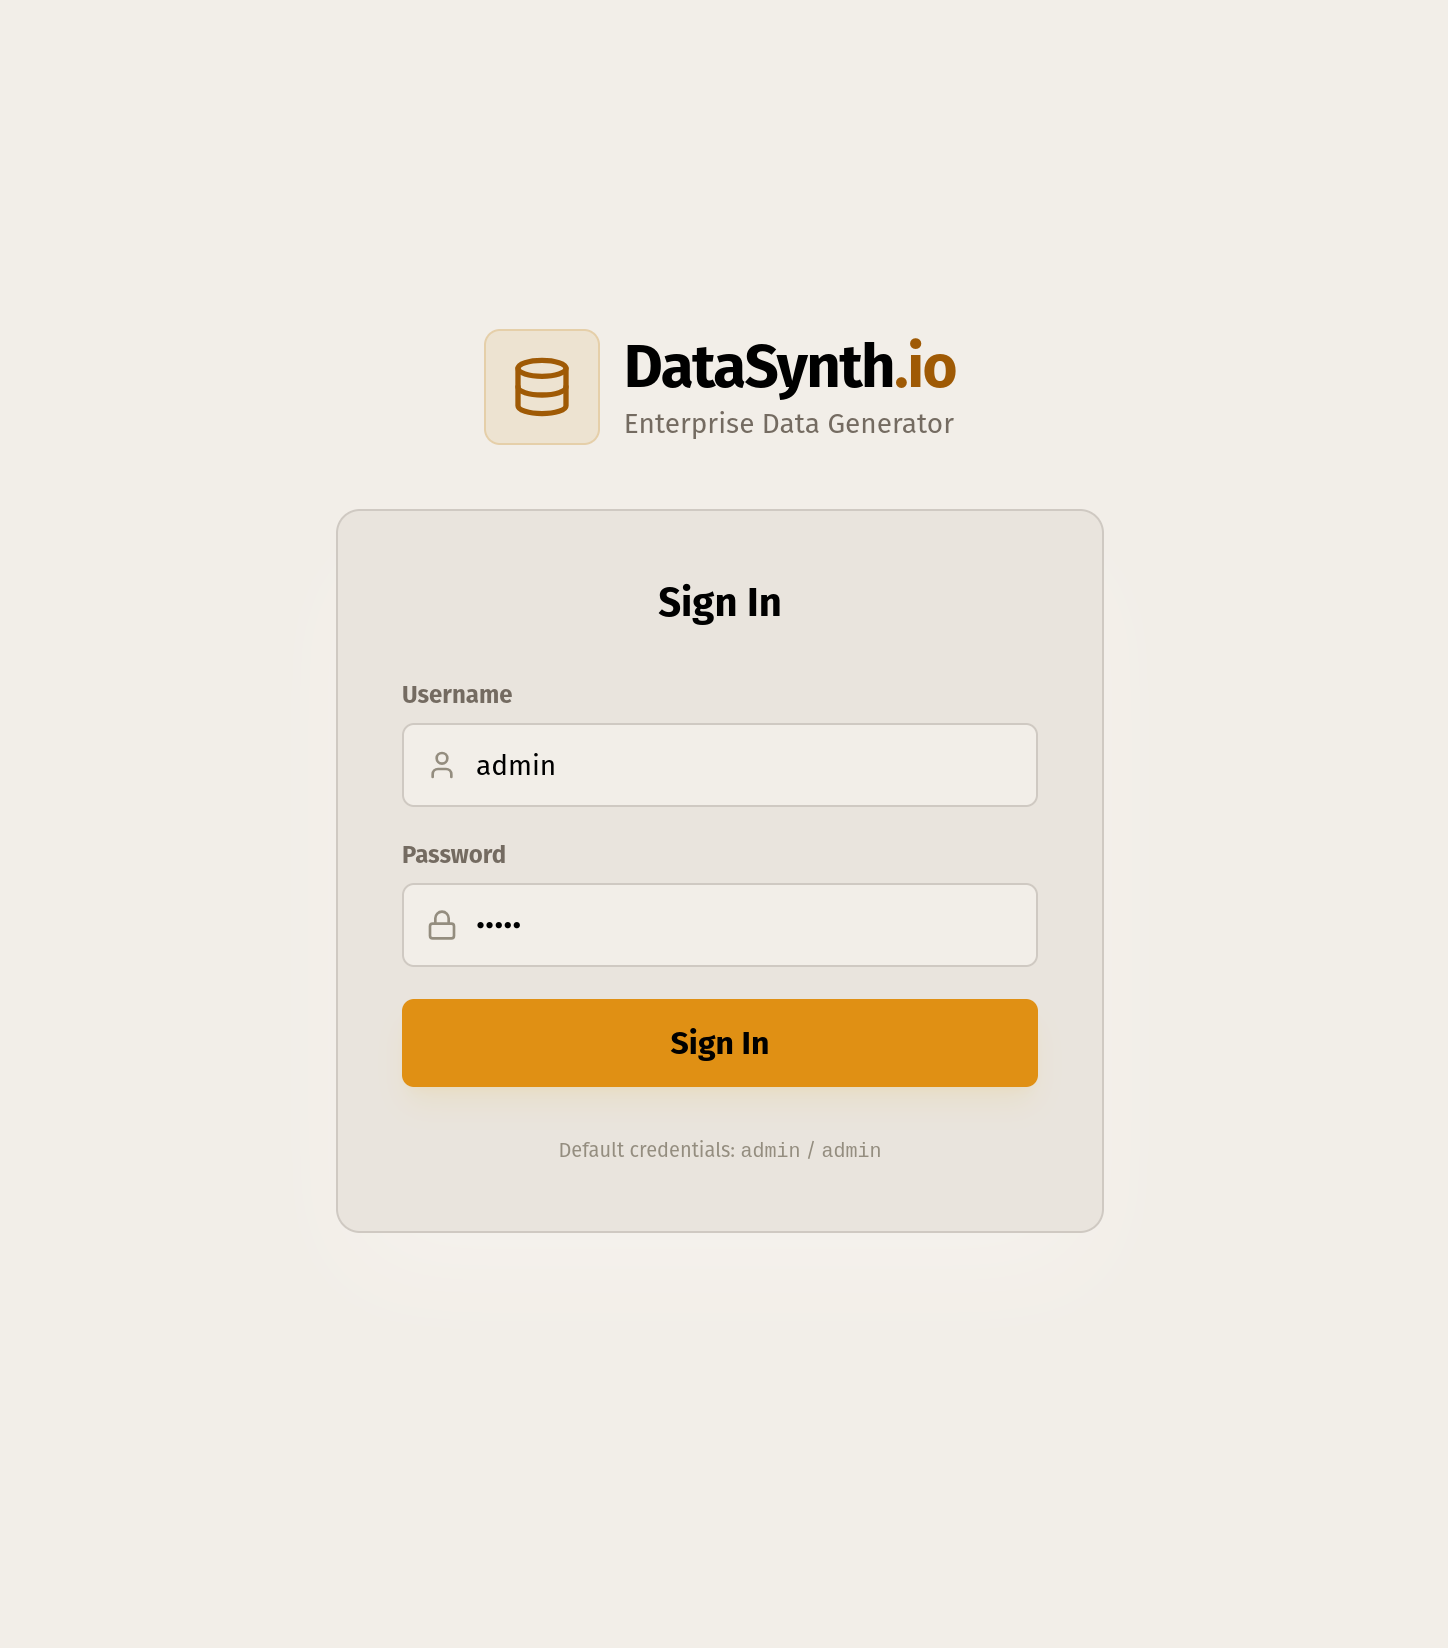
\includegraphics[width=0.8\textwidth]{images/login_page.png}
    \caption{Ekran logowania do systemu}
    \label{fig:login_page}
\end{figure}

Na rysunku \ref{fig:login_page} przedstawiono widok logowania. Użytkownik musi podać nazwę użytkownika oraz hasło. System komunikuje się z \gls{API} w celu weryfikacji poświadczeń i w przypadku sukcesu otrzymuje token \gls{JWT}, który jest zapisywany w pamięci przeglądarki. Interfejs obsługuje również wyświetlanie komunikatów o błędach w przypadku niepoprawnych danych.

\subsection*{Główny widok aplikacji}
Po zalogowaniu użytkownik dostaje dostęp do głównego widoku aplikacji, który stanowi centrum tworzenia schematu bazy danych. Interfejs został zaprojektowany z myślą o ergonomii, dzieląc ekran na dwie główne sekcje: lewy panel konfiguracyjny (budowanie schematu) oraz prawy panel wyników (podgląd i eksport). Opis obu części znajduje się poniżej.

Lewy panel zawiera zestaw narzędzi niezbędnych do zdefiniowania struktury zbioru danych. Składa się on z następujących kluczowych modułów:

\subsubsection*{1. Pasek narzędzi}
W górnej części panelu znajduje się pasek narzędzi służący do zarządzania stanem całego projektu. Użytkownik ma tutaj dostęp do następujących funkcjonalności:
\begin{itemize}
    \item Zarządzanie projektami: Przyciski umożliwiające zapisywanie i wczytywanie projektów z bazy danych.
    \item Szablony (Templates): Dostęp do gotowych, predefiniowanych schematów danych.
    \item Import/Eksport: Możliwość zapisania schematu do lokalnego pliku \gls{JSON} oraz jego ponownego wczytania.
    \item Wczytywanie przykładowych danych: Opcja pozwalająca na szybkie załadowanie przykładowego schematu (np. ,,E-commerce''), co jest szczególnie przydatne dla nowych użytkowników.
\end{itemize}

\subsubsection*{2. Konfiguracja globalna (Global Configuration)}
Poniżej paska narzędzi znajdują się parametry definiujące ogólne właściwości generowanego zbioru danych:
\begin{itemize}
    \item Nazwa zbioru: Pole tekstowe definiujące nazwę zadania, która później służy jako nazwa pliku wynikowego.
    \item Lokalizacja (Locale): Rozwijana lista pozwalająca wybrać krąg kulturowy generowanych danych (np. \texttt{en\_US}, \texttt{pl\_PL}, \texttt{de\_DE}). Wybór ten wpływa na formatowanie dat, walut, numerów telefonów oraz język generowanych tekstów przez bibliotekę Faker.
    \item Format wyjściowy: Pozwala zdefiniować, w jakiej postaci mają zostać zwrócone dane (\gls{JSON}, \gls{CSV} spakowany w ZIP, plik \gls{SQL}).
    \item Globalny kontekst AI: Pole tekstowe, w którym użytkownik może opisać ogólny charakter generowanych danych (np. ,,System medyczny dla szpitala wojewódzkiego''). Kontekst ten jest ,,doklejany'' do promptów wysyłanych do modeli \gls{LLM}, co pozwala na zachowanie spójności tematycznej wszystkich generowanych pól.
\end{itemize}

\begin{figure}[H]
    \centering
    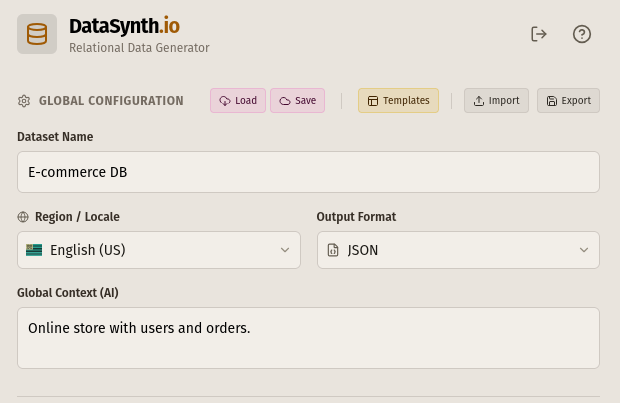
\includegraphics[width=0.8\textwidth]{images/global_config.png}
    \caption{Formularz konfiguracji globalnej i pasek narzędzi}
    \label{fig:global_config}
\end{figure}


\subsubsection*{3. Menedżer tabel (Table Manager)}
Poniżej konfiguracji znajduje się lista zdefiniowanych tabel. Moduł ten pozwala na:
\begin{itemize}
    \item Tworzenie struktur relacyjnych: Użytkownik może dodawać dowolną liczbę tabel, co pozwala na modelowanie złożonych relacji bazodanowych.
    \item Kontrolę wolumenu danych: Każda tabela posiada niezależny licznik wierszy, co pozwala np. wygenerować 100 użytkowników i 5000 zamówień.
    \item Przeglądanie tabel: Kliknięcie w nagłówek tabeli aktywuje ją, zmieniając kontekst dla listy pól i edytora.
\end{itemize}

\begin{figure}[H]
    \centering
    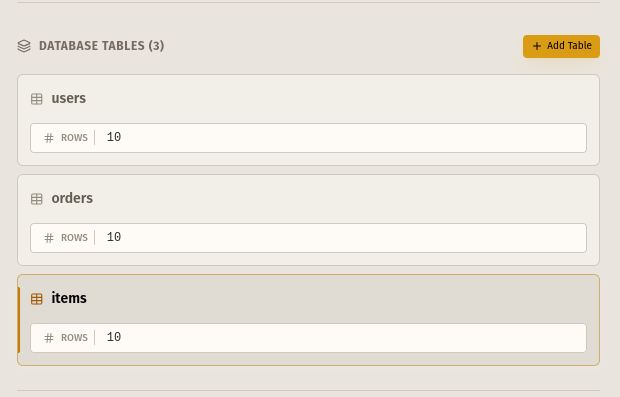
\includegraphics[width=0.65\textwidth]{images/tables.png}
    \caption{Menedżer tabel}
    \label{fig:tables}
\end{figure}


\subsubsection*{4. Kreator pól (Schema Builder)}
Kluczowym elementem interfejsu jest formularz dodawania nowych pól do tabeli.
\begin{figure}[H]
    \centering
    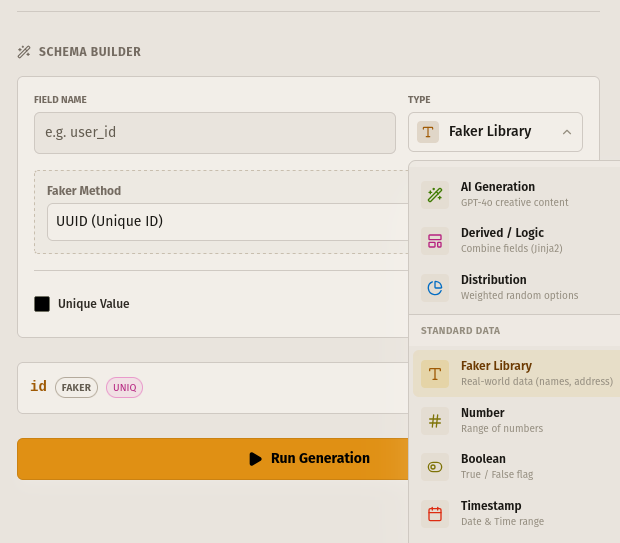
\includegraphics[width=0.8\textwidth]{images/schema_builder.png}
    \caption{Formularz definiowania nowego pola}
    \label{fig:schema_builder}
\end{figure}

Moduł ten (Rysunek \ref{fig:schema_builder}) dynamicznie dostosowuje dostępne parametry w zależności od wybranego typu danych. Użytkownik może:
\begin{itemize}
    \item Wybrać typ generatora (np. Faker, AI/\gls{LLM}, Integer, Foreign Key).
    \item Skonfigurować parametry specyficzne (np. zakres liczb, prompt dla AI, tabelę docelową dla klucza obcego).
    \item Oznaczyć pole jako unikalne (Unique), co wymusi generowanie niepowtarzalnych wartości.
\end{itemize}

Na rysunkach \ref{fig:schema_builder_ai} oraz \ref{fig:schema_builder_distribution} przedstawiono przykładowe konfiguracje dla generatora AI oraz generatora z rozkładem prawdopodobieństwa.

\begin{figure}[H]
    \centering
    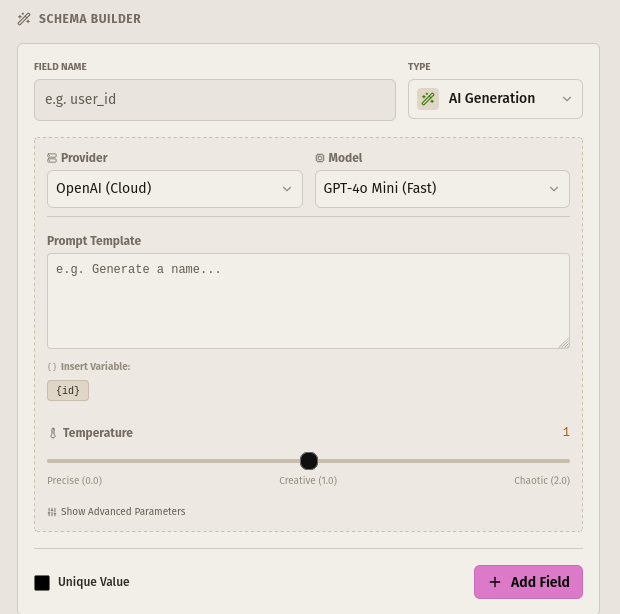
\includegraphics[width=0.8\textwidth]{images/schema_builder_ai.png}
    \caption{Formularz definiowania nowego pola z wykorzystaniem AI}
    \label{fig:schema_builder_ai}
\end{figure}

\begin{figure}[H]
    \centering
    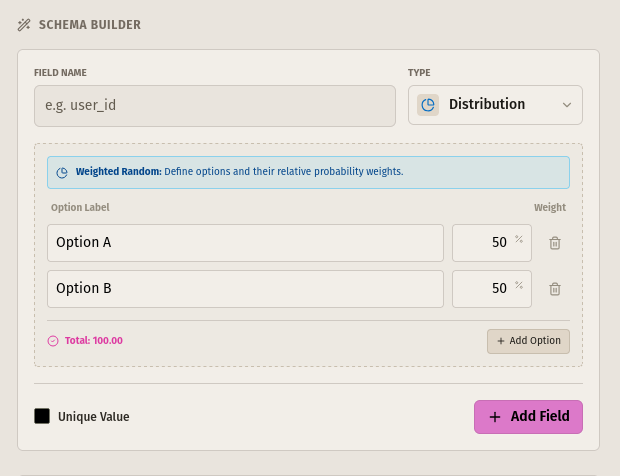
\includegraphics[width=0.8\textwidth]{images/schema_builder_distribution.png}
    \caption{Formularz definiowania nowego pola z wykorzystaniem rozkładu prawdopodobieństwa}
    \label{fig:schema_builder_distribution}
\end{figure}


\subsubsection*{5. Lista pól (Field List)}
Dolną część panelu zajmuje lista pól dla aktywnej tabeli. Każdy element listy prezentuje nazwę kolumny, typ generatora (oznaczony kolorowym badge'm dla łatwej identyfikacji) oraz ewentualne flagi (np. \texttt{UNIQ} dla wartości unikalnych). Moduł umożliwia również szybką edycję parametrów oraz usuwanie poszczególnych pól ze struktury.

\begin{figure}[H]
    \centering
    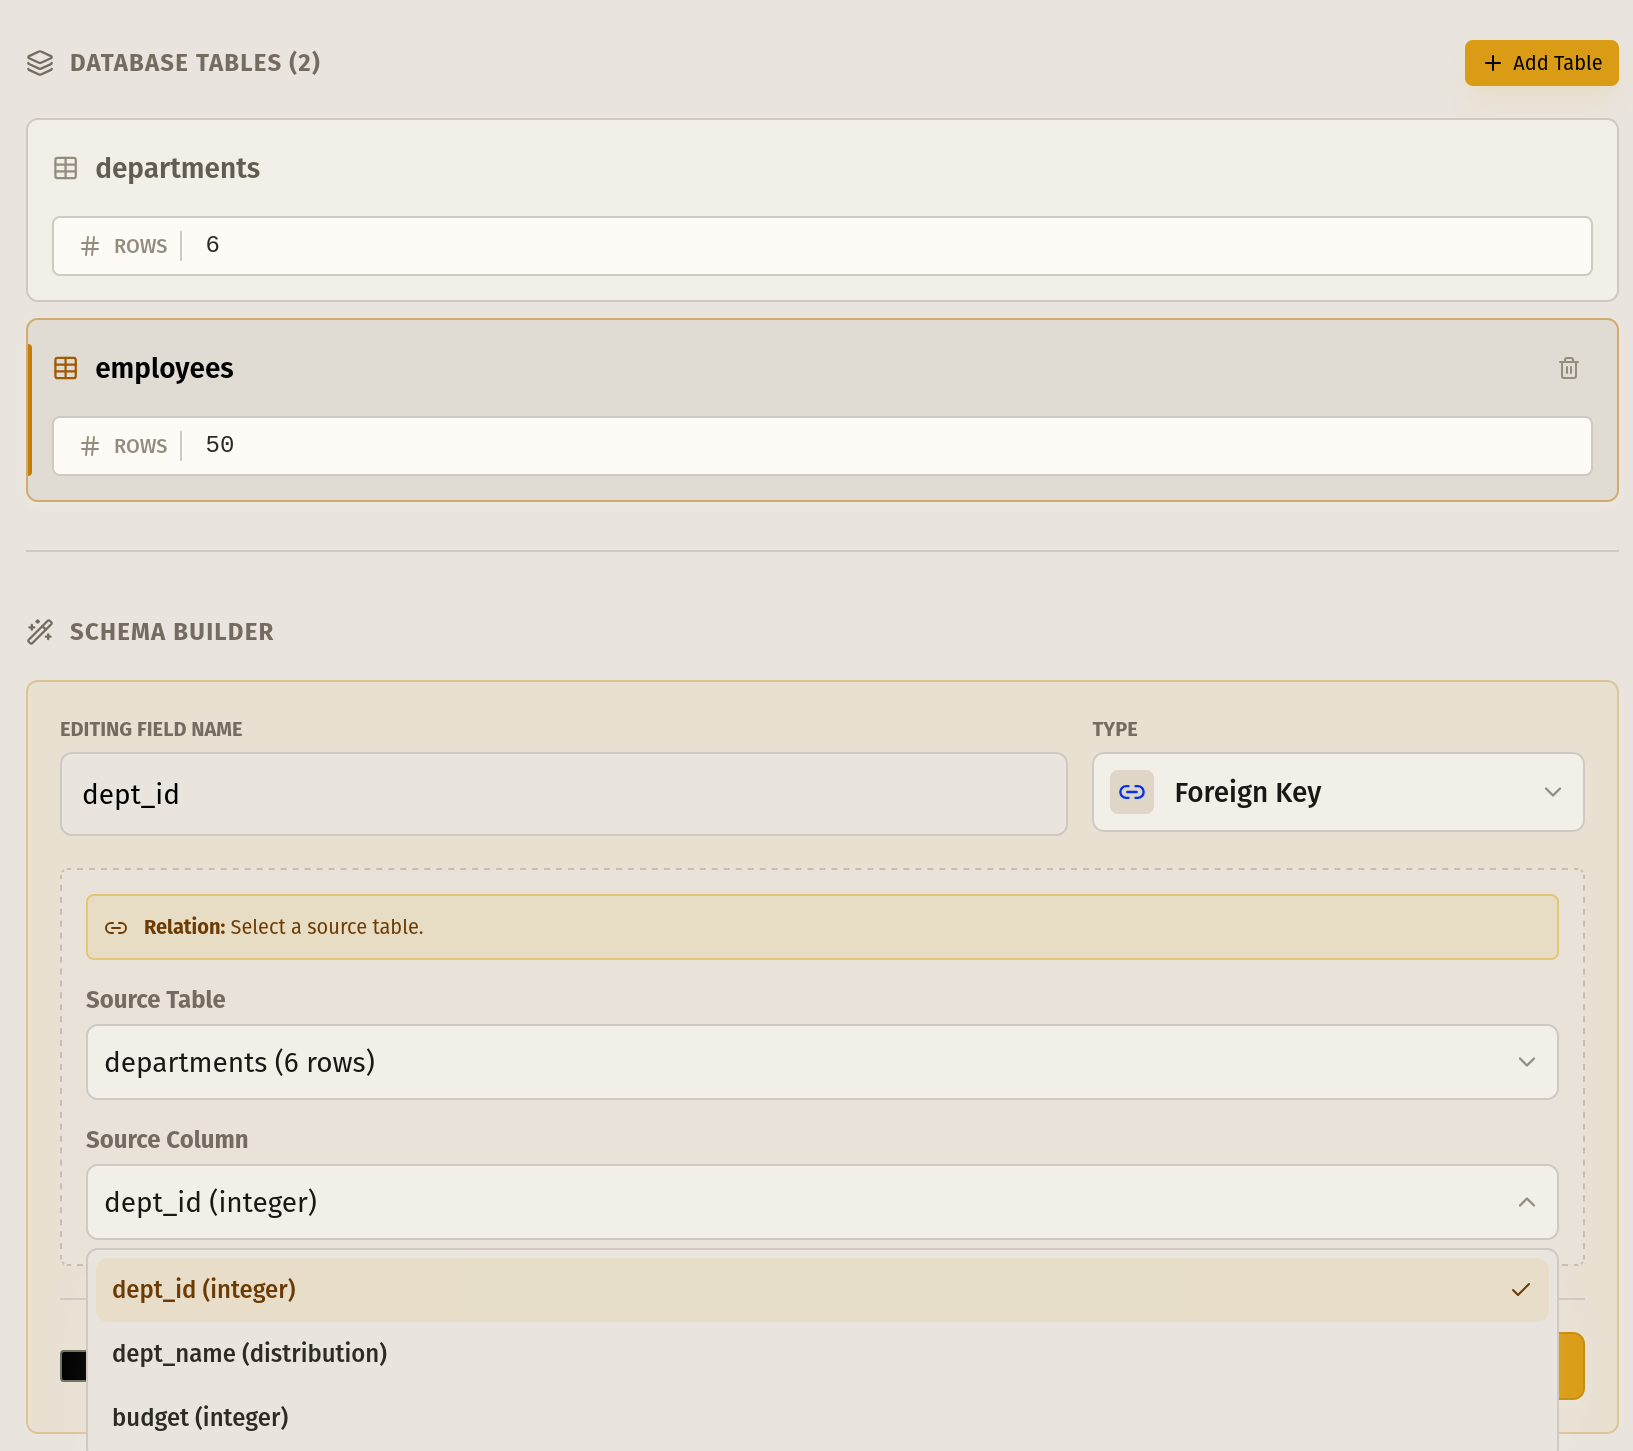
\includegraphics[width=0.85\textwidth]{images/foreign_key_screen.png}
    \caption{Interfejs konfigurowania klucza obcego pośród opcji parametrów w panelu bocznym}
    \label{fig:foreign_key_ui}
\end{figure}

Rysunek \ref{fig:foreign_key_ui} przedstawia zrzut ekranu panelu ustawień wybranego pola w kreatorze schematu. Po wskazaniu typu generatora klucza obcego, użytkownikowi automatycznie prezentowane są dedykowane parametry, pozwalające na wygodne wskazanie tabeli nadrzędnej oraz konkretnej kolumny (z wcześniej dodanych przez użytkownika pól). Rozwiązanie to zdejmuje z twórcy schematu ciężar konieczności manualnego wpisywania komend \gls{SQL}, znacznie ułatwiając sprawne i wizualne prototypowanie relacji między tabelami.

\begin{figure}[H]
    \centering
    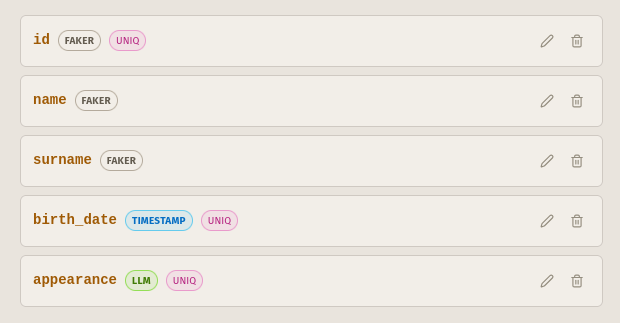
\includegraphics[width=0.8\textwidth]{images/field_list.png}
    \caption{Lista pól dla aktywnej tabeli}
    \label{fig:field_list}
\end{figure}

\subsection*{Generowanie i eksport danych}
Proces generowania danych odbywa się asynchronicznie, a postęp jest wizualizowany za pomocą paska postępu.

\begin{figure}[H]
    \centering
    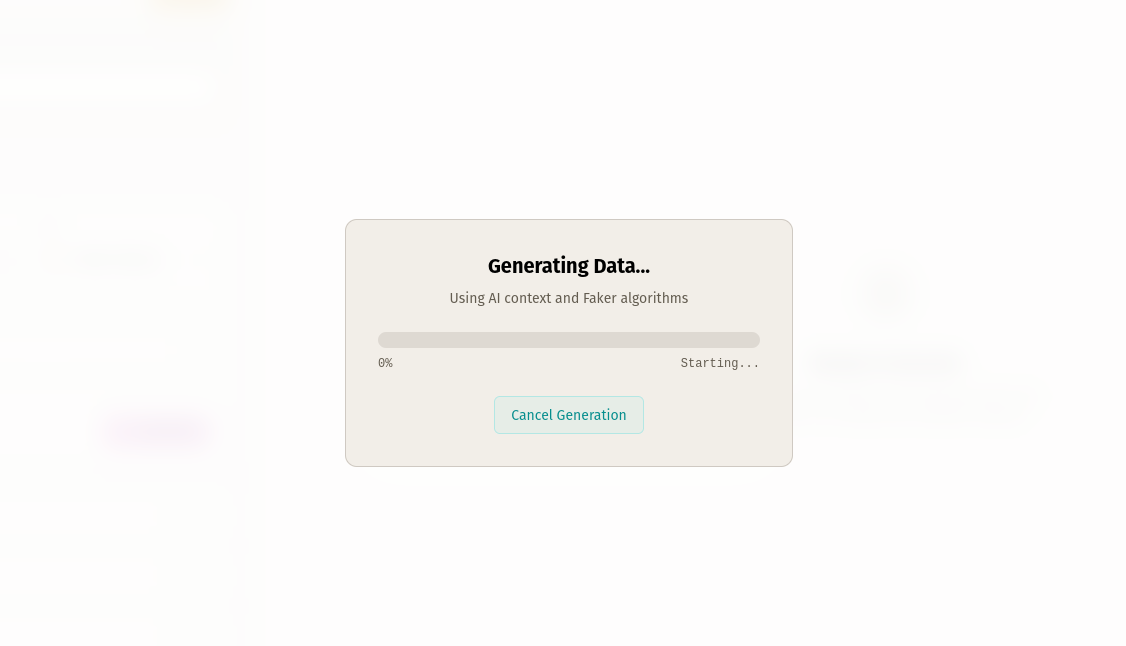
\includegraphics[width=1\textwidth]{images/loading.png}
    \caption{Okno postępu generowania}
    \label{fig:generation_modal}
\end{figure}

Po zakończeniu procesu (Rysunek \ref{fig:generation_modal}), wyniki są prezentowane w panelu wyjściowym. Użytkownik ma wtedy możliwość:
\begin{itemize}
    \item Przejrzenia wygenerowanych danych w formacie tabeli, jak i w formacie \gls{JSON} bezpośrednio w przeglądarce (wprowadzono ograniczenie do 100 wierszy, aby uniknąć problemów z wydajnością).
    \item Skopiowania widocznego fragmentu danych do schowka.
    \item Pobrania danych jako plik \gls{JSON}, \gls{SQL} lub pakiet \gls{CSV}.
    \item Bezpośredniego eksportu danych do zewnętrznej bazy danych (poprzez podanie parametrów połączenia).
\end{itemize}

% \begin{figure}[H]
%     \centering
%     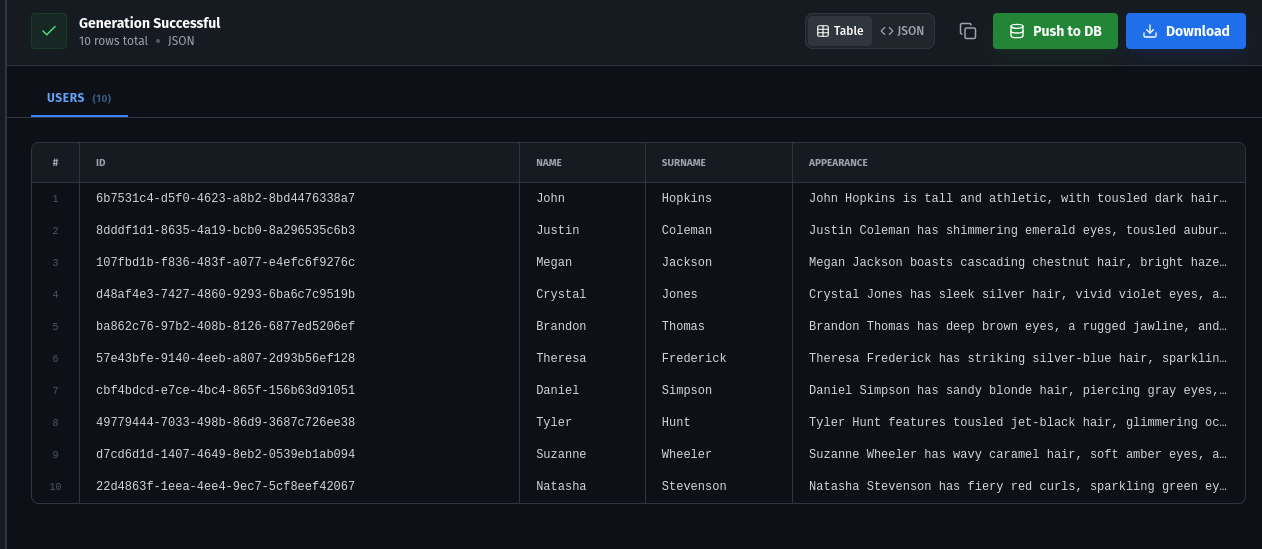
\includegraphics[width=0.7\textwidth]{images/generated_data_table.png}
%     \caption{Wygenerowane dane w formacie tabeli}
%     \label{fig:generated_data_table}
% \end{figure}

% \begin{figure}[H]
%     \centering
%     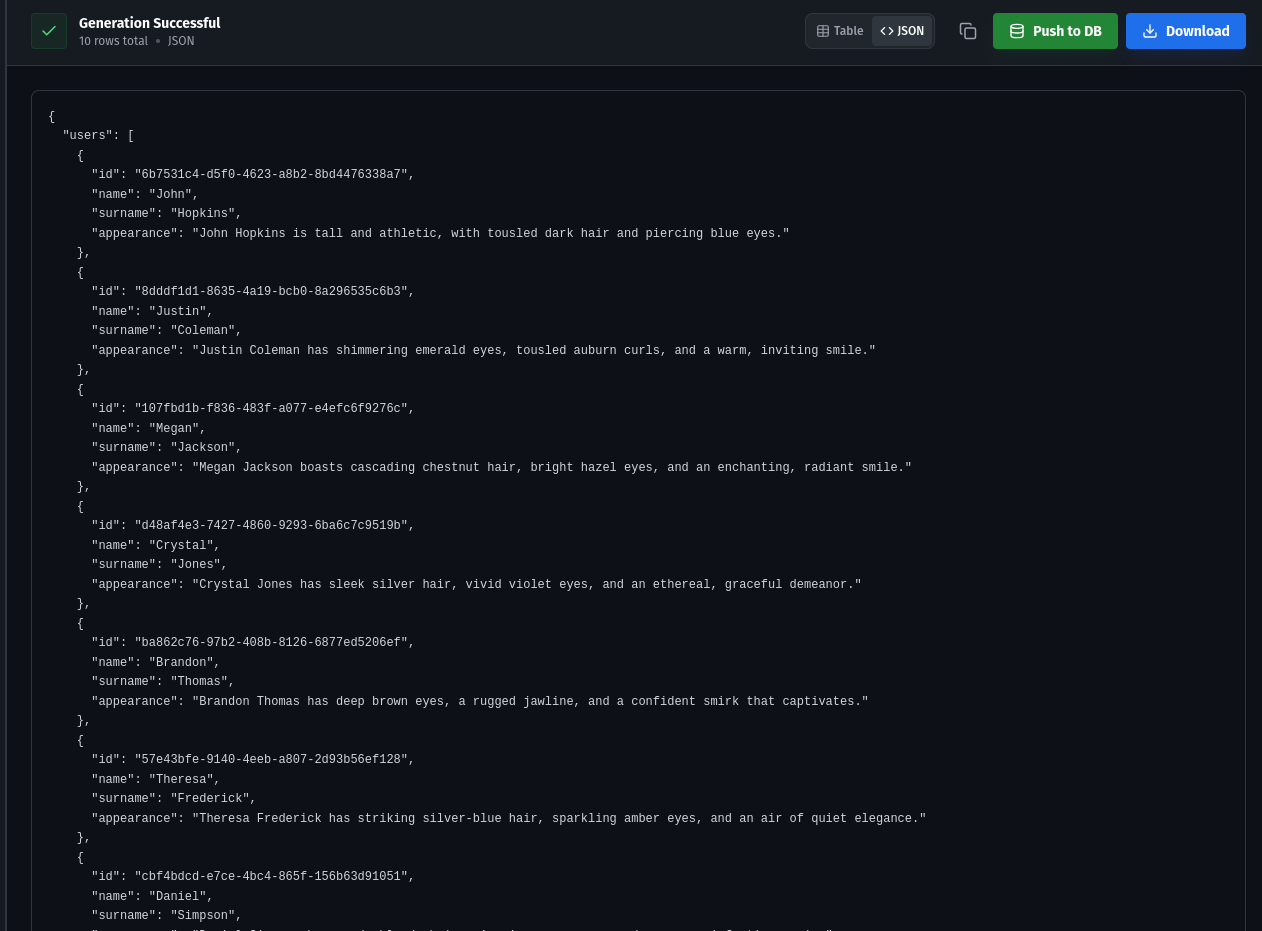
\includegraphics[width=0.7\textwidth]{images/generated_data_json.png}
%     \caption{Wygenerowane dane w formacie \gls{JSON}}
%     \label{fig:generated_data_json}
% \end{figure}

\begin{figure}[H]
    \centering
    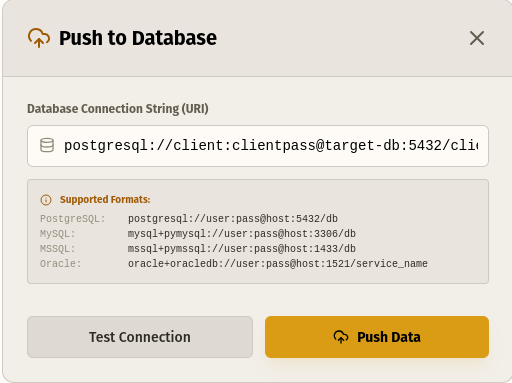
\includegraphics[width=0.7\textwidth]{images/push_to_database_modal.png}
    \caption{Okno eksportu danych do bazy danych}
    \label{fig:push_to_database_modal}
\end{figure}

Na rysunku \ref{fig:push_to_database_modal} przedstawiono formularz umożliwiający bezpośredni eksport danych do zewnętrznej bazy danych, co jest szczególnie przydatne dla deweloperów chcących szybko zasilić testową bazę danymi.

Z racji na zbyt duży rozmiar pliku, zrezygnowano z umieszczania zrzutów ekranu z widokiem wygenerowanych danych w pracy pisemnej.

Stan aplikacji jest zarządzany głównie przy użyciu hooków React (\texttt{useState}, \texttt{useEffect}). Do obsługi złożonego stanu edytora schematu stworzono dedykowany hook \texttt{useSchema}, który centralizuje logikę dodawania, usuwania i edycji tabel oraz pól.

Do komunikacji z backendem wykorzystano bibliotekę \texttt{axios}. Zaimplementowano instancję klienta \gls{API} (w pliku \texttt{api.js}), która automatycznie dołącza token autoryzacyjny do każdego żądania oraz obsługuje błędy odpowiedzi serwera (np. automatyczne wylogowanie po wygaśnięciu tokenu).

\section{Implementacja algorytmów}

\subsection*{Algorytm rozwiązywania zależności (sortowanie topologiczne)}
Aby zapewnić poprawność relacyjną generowanych danych, niezbędne jest ustalenie odpowiedniej kolejności przetwarzania tabel. Problem ten sprowadza się do posortowania wierzchołków skierowanego grafu zależności w taki sposób, aby dla każdej krawędzi $(u, v)$ wierzchołek $u$ pojawiał się przed wierzchołkiem $v$.

W systemie zaimplementowano wariant algorytmu Kahna dla sortowania topologicznego \cite{topological_sort}. Proces przebiega w następujących krokach:
\begin{enumerate}
    \item Budowa grafu zależności: Dla każdej tabeli analizowanem są jej pola. Jeśli pole jest typu \texttt{foreign\_key}, dodawana jest zależność od tabeli docelowej.
    \item Inicjalizacja: Tworzona jest lista tabel ,,gotowych'' (nieposiadających niewygenerowanych zależności).
    \item Iteracja: Dopóki lista ,,gotowych'' tabel nie jest pusta:
          \begin{itemize}
              \item Wybierana jest tabela, dodawana do listy wynikowej.
              \item Tabela ta jest usuwana z zależności innych tabel.
              \item Jeśli w wyniku usunięcia inna tabela traci wszystkie zależności, trafia na listę "gotowych".
          \end{itemize}
    \item Weryfikacja: Jeśli po zakończeniu algorytmu lista wynikowa jest krótsza niż całkowita liczba tabel, oznacza to wykrycie cyklu, co jest zgłaszane jako błąd.
\end{enumerate}

\subsection*{Integracja z LLM}
Generowanie danych przy użyciu \gls{LLM} odbywa się w metodzie \texttt{\_generate\_llm\_value}. Proces ten jest znacznie bardziej złożony niż proste wywołanie \gls{API}.

Prompt wysyłany do modelu składa się z trzech części:
\begin{itemize}
    \item System Message: Instruuje model, aby wcielił się w rolę generatora danych fikcyjnych.
    \item Szablon użytkownika: Szablon zdefiniowany przez użytkownika, np. ,,Opisz osobę \{name\} \{surname\}''. Zmienne w nawiasach klamrowych są podmieniane na wartości wygenerowane w bieżącym wierszu przy użyciu silnika Jinja2.
    \item Ograniczenia: Dodawane dynamicznie instrukcje, np. wymuszenie unikalności.
\end{itemize}

Zapewnienie unikalności w modelach probabilistycznych jest wyzwaniem. System stosuje podejście iteracyjne:
\begin{verbatim}
attempts = 0
while attempts < 10:
    temperature = base_temp + (attempts * 0.1)
    prompt = construct_prompt(template, avoid_values)
    context_injection(prompt, current_row_data)
    value = await call_llm(prompt, temperature)
    
    if is_unique(value):
        return value
    
    attempts += 1
\end{verbatim}
Temperatura (temperature) jest hiperparametrem kontrolującym losowość generowanych odpowiedzi \gls{LLM}. Wzrost temperatury w kolejnych próbach spłaszcza rozkład prawdopodobieństwa kolejnych słów, co zwiększa ,,kreatywność'' modelu i znacząco zmniejsza szansę na wygenerowanie duplikatu.

W celu optymalizacji wydajności generowania danych \gls{LLM}, zaimplementowano dwufazowy algorytm przetwarzania. W pierwszej fazie silnik generuje wszystkie pola deterministyczne (z parametrem \texttt{skip\_llm=True}), budując kontekst każdego wiersza. Następnie zebrane konteksty są przekazywane do metody \texttt{\_generate\_llm\_batch\_value}, która dzieli je na podpartie o stałym rozmiarze (\texttt{SUB\_BATCH\_SIZE}). Dla każdej podpartii formułowany jest zbiorczy prompt, a model jest instruowany, by zwrócił tablicę \gls{JSON} z odpowiedziami. Podpartie są przetwarzane współbieżnie z ograniczeniem przez \texttt{asyncio.Semaphore} (\texttt{MAX\_CONCURRENT} slotów). Szczegóły procesu optymalizacji i doboru parametrów opisano w Rozdziale~\ref{sec:llm_optimization}.

Do wizualizacji postępu w czasie rzeczywistym wykorzystano protokół WebSocket. Po nawiązaniu połączenia pod adresem \texttt{ws://server:8001/ws/jobs/\{job\_id\}}, serwer cyklicznie przesyła ramki \gls{JSON} o strukturze:

\begin{verbatim}
{
  "job_id": "9fa2204c-72d6-...",
  "status": "processing",  // lub "completed", "failed"
  "progress": 45,          // wartość procentowa 0-100
  "total_rows": 1000,
  "error": null            // ewentualny komunikat błędu
}
\end{verbatim}

Frontend (komponent \texttt{GenerationModal}) subskrybuje te wiadomości i na ich podstawie aktualizuje pasek postępu. Po otrzymaniu statusu \texttt{completed}, połączenie jest zamykane, a interfejs przechodzi do widoku wyników.

\section{Infrastruktura i konteneryzacja}
Całe środowisko uruchomieniowe zostało zdefiniowane w pliku \texttt{docker-compose.yml}. Definiuje on następujące serwisy:
\begin{itemize}
    \item \texttt{backend}: Kontener z aplikacją FastAPI.
    \item \texttt{frontend}: Kontener serwujący pliki statyczne aplikacji React (lub serwer developerski w trybie dev).
    \item \texttt{worker}: Kontener procesu Celery do zadań w tle.
    \item \texttt{db}: Baza danych PostgreSQL dla aplikacji.
    \item \texttt{redis}: Broker wiadomości dla Celery.
    \item \texttt{target-db}: Dodatkowa instancja PostgreSQL, służąca jako przykładowa docelowa baza danych do bezpośredniego zasilania danymi.
    \item \texttt{ollama}: Usługa serwująca modele \gls{LLM}.
\end{itemize}

Dzięki takiemu podejściu, uruchomienie całego systemu sprowadza się do wykonania jednego polecenia \texttt{docker compose up}, co znacząco upraszcza proces instalacji i testowania rozwiązania.